\section{Conversions}
\label{Se:Conversions}


It is possible to both convert from a WALi WPDS to an NWA and from an NWA to
a WPDS.  However, the construction of an NWA from a WPDS is not the inverse
of constructing a WPDS from an NWA, i.e., one cannot perform the two
conversions in sequence and obtain the identity conversion.

At a high level, these operations work by making the NWA track both the state
of the PDS and it's top-of-stack symbol. A PDS rule of the form $\langle
p,q_1 \rangle \hookrightarrow \langle p,q_2 \rangle$ leaves the stack height
unchanged, and thus is associated with an internal NWA transition; in this
case, that transition goes from the state $(p,q_1)$ to $(p,q_2)$. The symbol
of a transition is associated with the top-of-stack symbol of the source
state, so in this example, the symbol labeling that transition would be
$q_1$. PDS push rules correspond to NWA call transitions, and PDS pop rules
correspond to NWA return transitions.

(This association is strongly informed by our uses of both PDSs and NWAs in
program analysis. It is common for PDSs to have just one state, $p$, and to
use the top-of-stack symbol to track the ``current'' program point. Pushing
something onto the stack corresponds to a call, and popping corresponds to a
return. For NWAs, we use the states themselves to track the current program
point. Furthermore, in our uses the labels on edges have been an identifier
for the program point the edge emanates from.)


\noindent The following operations are methods of class NWA:

\begin{description}

  \item\texttt{WPDS plusWPDS( const WPDS\& base )} \nopagebreak

    This operation is an instance method.  It returns the WPDS that is the
    product of the NWA referred to by \texttt{this} and the given WPDS
    \cite{advancedquerying}.

  \item\texttt{void PDStoNWA( const WPDS\& pds )} \nopagebreak

    This operation is an instance method; the NWA referred to by
    \texttt{this} is converted to the NWA that is equivalent to the given
    PDS.  Typical sequence of operations:
    construct A; A.PDStoNWA(pds);

  \item\texttt{static ref\_ptr<NWA> PDStoNWA( const WPDS\& pds )} \nopagebreak

    Constructs and returns the NWA that is equivalent to the given PDS.

  \item\texttt{WPDS NWAtoPDScalls( WeightGen<Client>\& wg ) const} \nopagebreak

    This operation is an instance method.  It constructs the WPDS that keeps
    call states on the stack that is equivalent to the NWA referred to by
    \texttt{this}.  It uses \texttt{wg} to determine weights for WPDS rules
    (see Section \ref{Se:NWAtoPDS}).

  \item\texttt{WPDS NWAtoBackwardsPDScalls( WeightGen<Client>\& wg ) const} \nopagebreak

    This operation is an instance method.  It constructs the backwards WPDS
    that keeps call states on the stack that is equivalent to the NWA
    referred to by \texttt{this}.  It uses \texttt{wg} to determine weights
    for WPDS rules (see Section \ref{Se:NWAtoPDS}).

  \item\texttt{WPDS NWAtoPDSreturns( WeightGen<Client>\& wg ) const} \nopagebreak

    This operation is an instance method.  It constructs the WPDS that keeps
    return states on the stack thatis equivalent to the NWA referred to by
    \texttt{this}.  It uses \texttt{wg} to determine weights for WPDS rules
    (see Section \ref{Se:NWAtoPDS}).  (Deprecated)

  \item\texttt{WPDS NWAtoBackwardsPDSreturns( WeightGen<Client>\& wg ) const} \nopagebreak

    This operation is an instance method.  It constructs the backwards WPDS
    that keeps return states on the stack that is equivalent to the NWA
    referred to by \texttt{this}.  It uses \texttt{wg} to determine weights
    for WPDS rules (see Section \ref{Se:NWAtoPDS}).  (Deprecated) \\

\end{description}


\subsection{PDS to NWA}
\label{Se:PDStoNWA}

The \texttt{PDStoNWA} functions convert a PDS into an NWA in a manner
faithful to the association suggested in the introduction to this section.

Formally, the conversion proceeds as follows:
\begin{enumerate}

\item For each $\langle p,q \rangle \hookrightarrow \langle p',q' \rangle \in
  \Delta_1$ in the PDS, we add $( (p,q), q, (p',q') )$ to the NWA's $\delta_i$

\item For each $\langle p,q_c \rangle \hookrightarrow \langle
  p',q_e \hspace{.1cm} q_r \rangle \in \Delta_2$ in the PDS, we add $(
  (p,q_c), q_c, (p',q_e) )$ to the NWA's $\delta_c$

\item For each $\langle p'',q_x \rangle \hookrightarrow \langle p''',\epsilon
  \rangle \in \Delta_0$ in the PDS, we add $( (p'',q_x), (p,q_c), q_x,
  (p''',q_r) )$ to the NWA's $\delta_r$ for all $(q_c,q_r)$ pairs such that
  $\langle p,q_c \rangle \hookrightarrow \langle p',q_e \hspace{.1cm} q_r
  \rangle \in \Delta_2$.

\end{enumerate}

\begin{figure}[p]
  \centering
    \begin{description}
      \centering
      \item $\langle p,main \rangle \hookrightarrow \langle p,q_1 \rangle$
      \item $\langle p,q_1 \rangle \hookrightarrow \langle p,c_1 \rangle$
      \item $\langle p,c_1 \rangle \hookrightarrow \langle p,e \hspace{.1cm} r_1 \rangle$
      \item $\langle p,e \rangle \hookrightarrow \langle p,q_2 \rangle$
      \item $\langle p,q_2 \rangle \hookrightarrow \langle p,q_3 \rangle$
      \item $\langle p,q_3 \rangle \hookrightarrow \langle p,x \rangle$
      \item $\langle p,x \rangle \hookrightarrow \langle p,\epsilon \rangle$
      \item $\langle p,r_1 \rangle \hookrightarrow \langle p,q_4 \rangle$
      \item $\langle p,q_4 \rangle \hookrightarrow \langle p,q_5 \rangle$
      \item $\langle p,q_5 \rangle \hookrightarrow \langle p,c_2 \rangle$
      \item $\langle p,c_2 \rangle \hookrightarrow \langle p,e \hspace{.1cm} r_2 \rangle$
      \item $\langle p,r_2 \rangle \hookrightarrow \langle p,q_6 \rangle$
      \item $\langle p,q_6 \rangle \hookrightarrow \langle p,exit \rangle$
    \end{description}
  \caption{An example PDS.}
  \label{Fig:PDStoNWA1}
\end{figure}

For example, the NWA resulting from converting the PDS shown in Figure
\ref{Fig:PDStoNWA1} into an NWA is shown in Figure \ref{Fig:PDStoNWA2}.

\begin{figure}[p]
  \centering
    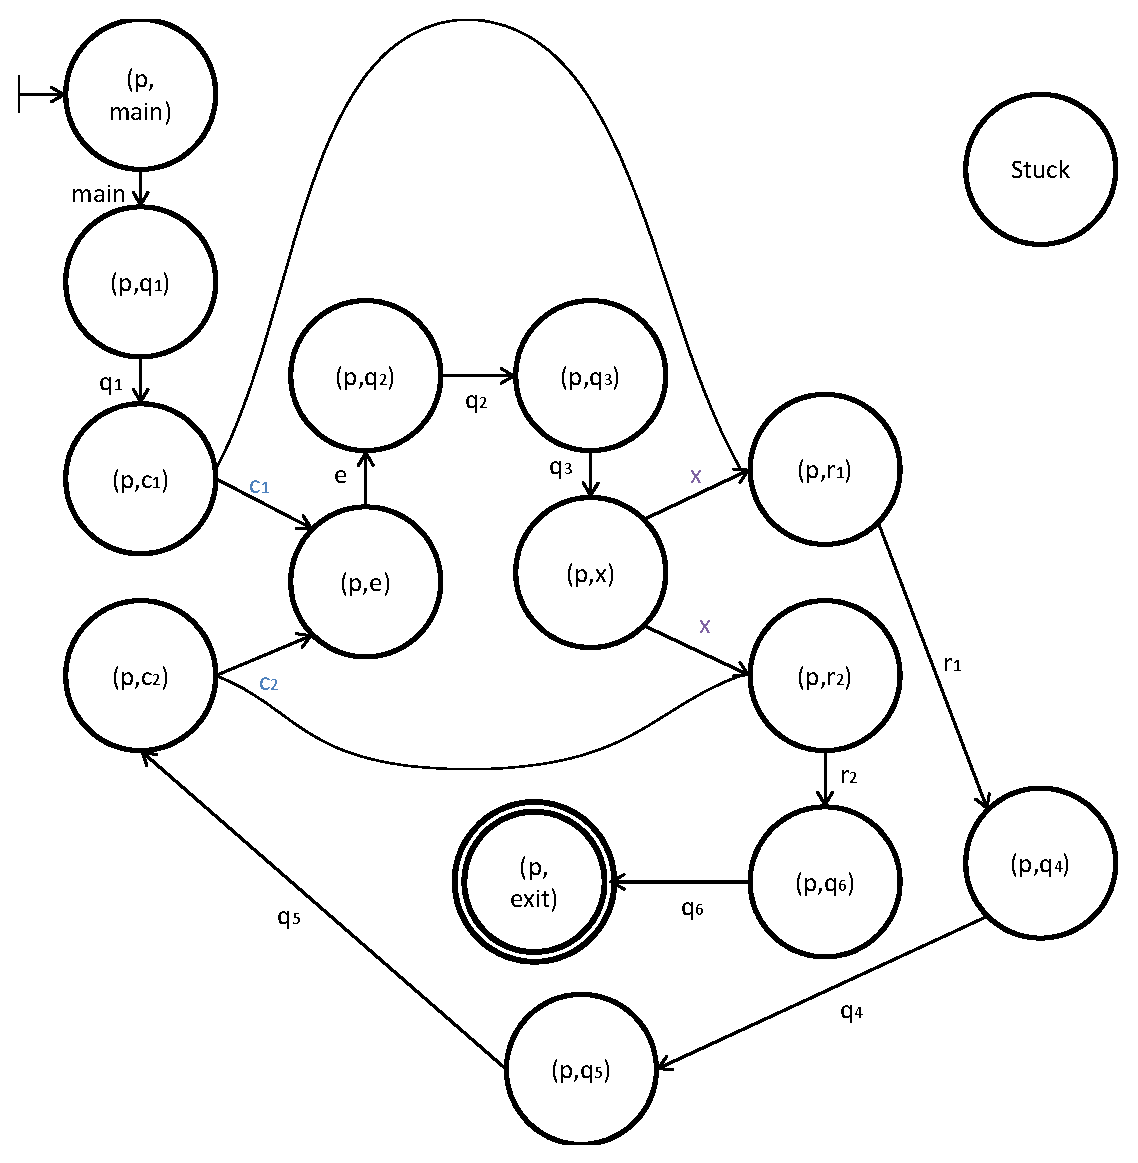
\includegraphics[width=12cm]{Figures/Figure22}
  \caption{The NWA resulting from converting the PDS in Figure \ref{Fig:PDStoNWA1} into an NWA.}
  \label{Fig:PDStoNWA2}
\end{figure}

The client information for all states in the resulting NWA are set to \texttt{null}.


\subsection{NWA to PDS}
\label{Se:NWAtoPDS}

An NWA can also be converted into a WPDS.  In this way it is possible to use
the reachability queries that are a part of the main WALi library on NWAs.
There are four variations on the NWA to WPDS
conversion: \begin{inparaenum} \item forward flow with call states on the
  stack \item backward flow with call states on the stack \item forward flow
  with return states on the stack \item backward flow with return states on
  the stack. \end{inparaenum} All four variations use \texttt{WeightGen} to
determine weights for WPDS rules.

\texttt{WeightGen} provides an abstract class that client code must implement for
calculating the weights for NWA transitions which are subsequently used in
calculating the weights for corresponding WPDS rules.  It allows the
underlying NWA to be decoupled from the weight domain used in the PDS.  See
\cite[\S4-\S5]{wali} for details about weight domains.


\noindent The following operations are methods of class WeightGen and are intended to be overridden:

\begin{description} 
  \item \texttt{sem\_elem\_t getOne()}  \nopagebreak
    Returns an instance of the $\bar{1}$ element of the weight domain.

  \item \texttt{sem\_elem\_t getWeight( Key source, ref\_ptr<ClientInfo> sourceInfo, \\  
                              \hspace*{3.25cm} Key symbol, Kind k, \\
                              \hspace*{3.25cm} Key target, ref\_ptr<ClientInfo> targetInfo )}  \nopagebreak
    Computes and returns the weight (in the desired semiring) for a
    (\texttt{kind}) NWA transition from \texttt{source} to \texttt{target}
    labeled with symbol \texttt{symbol}.

  \item \texttt{sem\_elem\_t getWildWeight( \\
                              \hspace*{3.25cm} Key source, ref\_ptr<ClientInfo> sourceInfo, \\
                              \hspace*{3.25cm} Key target, ref\_ptr<ClientInfo> targetInfo )}  \nopagebreak
    Computes and returns the weight (in the desired semiring) for an NWA
    transition from \texttt{source} to \texttt{target} labeled with the
    meta-symbol \texttt{*}. \\
\end{description}

(By default, \texttt{getWeight} and \texttt{getWildWeight} return the result
of a call to \texttt{getOne}, so the only function that absolutely needs to be
overridden is \texttt{getOne}. This is pure virtual in \texttt{WeightGen}, so
the compiler will not let you ignore this responsibility.)


\begin{figure}[htbp]
  \centering
    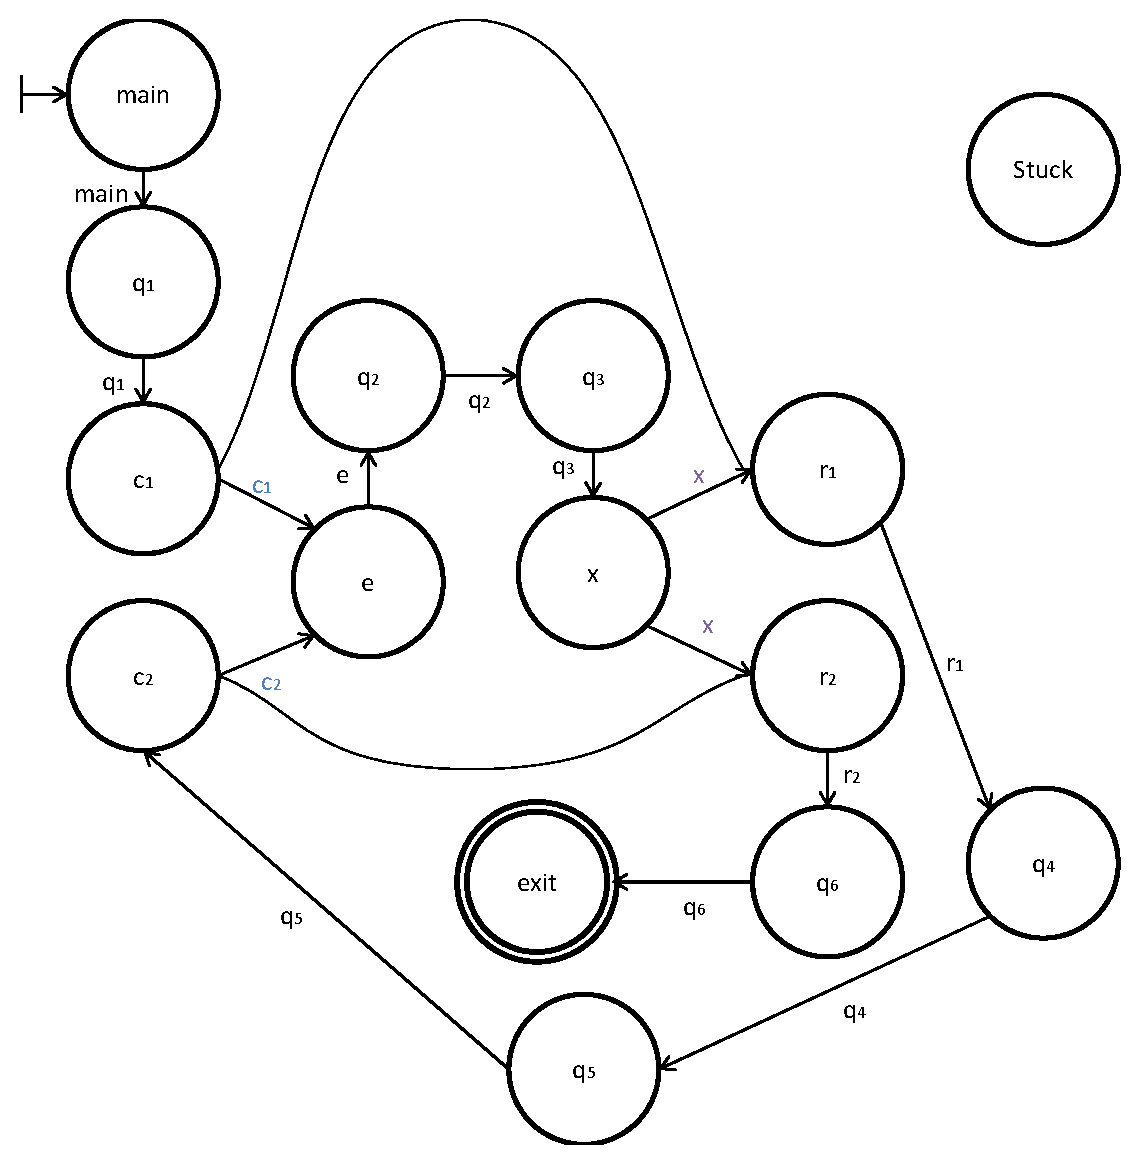
\includegraphics[width=12cm]{Figures/Figure23}
  \caption{An example NWA.}
  \label{Fig:NWAtoPDS1}
\end{figure}

\subsubsection{1. Forwards Flow Stacking Calls}

\noindent The conversion is performed by:

\begin{enumerate}

\item For each $(q,\sigma,q')$ $\in \delta_i$ in the NWA, adding $\langle p,q
  \rangle \hookrightarrow \langle p,q' \rangle$ to $\Delta_1$ of the WPDS
  (with weight
  \texttt{wg.getWeight($q$,$CI_q$,$\sigma$,INTRA,$q'$,$CI_{q'}$}) or
  \texttt{wg.getWildWeight($q$,$CI_q$,$q'$,$CI_{q'}$)}, depending on
  $\sigma$).

\item For each $(q_c,\sigma, q_e)$ $\in \delta_c$ in the NWA, adding $\langle
  p,q_c \rangle \hookrightarrow \langle p, q_e \hspace{.1cm} q_c \rangle$ to
  $\Delta_2$ of the WPDS (with weight
  \texttt{wg.getWeight($q_c$,$CI_{q_c}$,$\sigma$,CALL\_TO\_ENTRY,$q_e$,$CI_{q_e}$)}
  or \texttt{wg.getWildWeight($q_c$,$CI_{q_c}$,$q_e$,$CI_{q_e}$)}, depending
  on $\sigma$).

\item For each $(q_x,q_c,\sigma,q_r)$ $\in \delta_r$ in the NWA, adding
  $\langle p,q_x \rangle \hookrightarrow \langle p_{q_x},\epsilon \rangle$ to
  $\Delta_0$ of the WPDS (with weight
  \texttt{wg.getWeight($q_x$,$CI_{q_x}$,$\sigma$,EXIT\_TO\_RET,$q_r$,$CI_{q_r}$)}
  or \texttt{wg.getWildWeight($q_x$,$CI_{q_x}$,$q_r$,$CI_{q_r}$)}, depending
  on $\sigma$) and $\langle p_{q_x},q_c \rangle \hookrightarrow \langle p,q_r
  \rangle$ to $\Delta_1$ of the WPDS (with weight \texttt{wg.getOne()}).

\end{enumerate}

\noindent Consider, as an example, converting the NWA in Figure
\ref{Fig:NWAtoPDS5} into a WPDS. The WPDS resulting from converting the PDS
shown in Figure \ref{Fig:NWAtoPDS1} into a WPDS is shown in Figure
\ref{Fig:NWAtoPDS4}. \\

\begin{figure}[htbp]
  \centering
    \begin{description}
      \centering
      \item $\langle p,main \rangle \hookrightarrow \langle p,q_1 \rangle$
      \item $\langle p,q_1 \rangle \hookrightarrow \langle p,c_1 \rangle$
      \item $\langle p,e \rangle \hookrightarrow \langle p,q_2 \rangle$
      \item $\langle p,q_2 \rangle \hookrightarrow \langle p,q_3 \rangle$
      \item $\langle p,q_3 \rangle \hookrightarrow \langle p,x \rangle$
      \item $\langle p,r_1 \rangle \hookrightarrow \langle p,q_4 \rangle$
      \item $\langle p,q_4 \rangle \hookrightarrow \langle p,q_5 \rangle$
      \item $\langle p,q_5 \rangle \hookrightarrow \langle p,c_2 \rangle$
      \item $\langle p,r_2 \rangle \hookrightarrow \langle p,q_6 \rangle$
      \item $\langle p,q_6 \rangle \hookrightarrow \langle p,exit \rangle$
      \item $\langle p,c_1 \rangle \hookrightarrow \langle p,e \hspace{.1cm} c_1 \rangle$
      \item $\langle p,c_2 \rangle \hookrightarrow \langle p,e \hspace{.1cm} c_2 \rangle$
      \item $\langle p,x \rangle \hookrightarrow \langle p_x, \epsilon \rangle$
      \item $\langle p_x,c_1 \rangle \hookrightarrow \langle p,r_1 \rangle$
      \item $\langle p,x \rangle \hookrightarrow \langle p_x, \epsilon \rangle$
      \item $\langle p_x,c_2 \rangle \hookrightarrow \langle p,r_2 \rangle$
    \end{description}
  \caption{The PDS resulting from converting the NWA shown in Figure \ref{Fig:NWAtoPDS1} into a PDS.}
  \label{Fig:NWAtoPDS4}
\end{figure}

\subsubsection{2. Backwards Flow Stacking Calls}

\noindent The conversion is performed by:

\begin{enumerate}

\item For each $(q,\sigma,q')$ $\in \delta_i$ in the NWA, adding $\langle
  p,q' \rangle \hookrightarrow \langle p,q \rangle$ to $\Delta_1$ of the WPDS
  (with weight
  \texttt{wg.getWeight($q$,$CI_q$,$\sigma$,INTRA,$q'$,$CI_{q'}$}) or
  \texttt{wg.getWildWeight($q$,$CI_q$,$q'$,$CI_{q'}$)}, depending on
  $\sigma$).

\item For each $(q_c,\sigma, q_e)$ $\in \delta_c$ and $(q_x,q_c,\gamma,q_r)$
  $\in \delta_r$ in the NWA, adding $\langle p,q_e \rangle \hookrightarrow
  \langle p_{q_e},\epsilon \rangle$ to $\Delta_0$ of the WPDS (with weight
  \texttt{wg.getWeight($q_c$,$CI_{q_c}$,$\sigma$,CALL\_TO\_ENTRY,$q_e$,$CI_{q_e}$)}
  or \texttt{wg.getWildWeight($q_c$,$CI_{q_c}$,$q_e$,$CI_{q_e}$)}, depending
  on $\sigma$) and $\langle p_{q_e},q_r \rangle \hookrightarrow \langle p,q_c
  \rangle$ to $\Delta_1$ of the WPDS (with weight \texttt{wg.getOne()} ).

\item For each $(q_x,q_c,\sigma,q_r) \in \delta_r$ in the NWA, adding
  $\langle p,q_r \rangle \hookrightarrow \langle p,q_x \hspace{.1cm} q_r
  \rangle$ to $\Delta_2$ of the WPDS (with weight
  \texttt{wg.getWeight($q_x$,$CI_{q_x}$,$\sigma$,EXIT\_TO\_RET,$q_r$,$CI_{q_r}$)}
  or \texttt{wg.getWildWeight($q_x$,$CI_{q_x}$,$q_r$,$CI_{q_r}$)}, depending
  on $\sigma$).

\end{enumerate}

\noindent Consider, as an example, converting the NWA in Figure
\ref{Fig:NWAtoPDS1} into a backwards flow WPDS.  The WPDS resulting from
converting the PDS shown in Figure \ref{Fig:NWAtoPDS1} into a backwards flow
WPDS is shown in Figure \ref{Fig:NWAtoPDS5}.  Note:
\texttt{NWAtoBackwardsPDScalls(A)} = \texttt{NWAtoPDScalls(reverse(A))}.  \\

\begin{figure}[htbp]
  \centering
    \begin{description}
      \centering
      \item $\langle p,q_1 \rangle \hookrightarrow \langle p,main \rangle$
      \item $\langle p,c_1 \rangle \hookrightarrow \langle p,q_1 \rangle$
      \item $\langle p,q_2 \rangle \hookrightarrow \langle p,e \rangle$
      \item $\langle p,q_3 \rangle \hookrightarrow \langle p,q_2 \rangle$
      \item $\langle p,x \rangle \hookrightarrow \langle p,q_3 \rangle$
      \item $\langle p,q_4 \rangle \hookrightarrow \langle p,r_1 \rangle$
      \item $\langle p,q_5 \rangle \hookrightarrow \langle p,q_4 \rangle$
      \item $\langle p,c_2 \rangle \hookrightarrow \langle p,q_5 \rangle$
      \item $\langle p,q_6 \rangle \hookrightarrow \langle p,r_2 \rangle$
      \item $\langle p,exit \rangle \hookrightarrow \langle p,q_6 \rangle$
      \item $\langle p,r_1 \rangle \hookrightarrow \langle p,x \hspace{.1cm} r_1 \rangle$
      \item $\langle p,r_2 \rangle \hookrightarrow \langle p,x \hspace{.1cm} r_2 \rangle$
      \item $\langle p,e \rangle \hookrightarrow \langle p_e, \epsilon \rangle$
      \item $\langle p_e,r_1 \rangle \hookrightarrow \langle p,c_1 \rangle$
      \item $\langle p,e \rangle \hookrightarrow \langle p_e, \epsilon \rangle$
      \item $\langle p_e,r_2 \rangle \hookrightarrow \langle p,c_2 \rangle$
    \end{description}
  \caption{The PDS resulting from converting the NWA shown in Figure \ref{Fig:NWAtoPDS1} into a PDS.}
  \label{Fig:NWAtoPDS5}
\end{figure}

\subsubsection{3. Forwards Flow Stacking Returns}

\noindent The conversion is performed by:

\begin{enumerate}

\item For each $(q,\sigma,q')$ $\in \delta_i$ in the NWA, adding $\langle p,q
  \rangle \hookrightarrow \langle p,q' \rangle$ to $\Delta_1$ of the WPDS
  (with weight
  \texttt{wg.getWeight($q$,$CI_q$,$\sigma$,INTRA,$q'$,$CI_{q'}$}) or
  \texttt{wg.getWildWeight($q$,$CI_q$,$q'$,$CI_{q'}$)}, depending on
  $\sigma$).

\item For each $(q_c,\sigma, q_e)$ $\in \delta_c$ and $(q_x,q_c,\gamma,q_r)$
  $\in \delta_r$ in the NWA, adding $\langle p,q_c \rangle \hookrightarrow
  \langle p, q_e \hspace{.1cm} q_r \rangle$ to $\Delta_2$ of the WPDS (with
  weight
  \texttt{wg.getWeight($q_c$,$CI_{q_c}$,$\sigma$,CALL\_TO\_ENTRY,$q_e$,$CI_{q_e}$)}
  or \texttt{wg.getWildWeight($q_c$,$CI_{q_c}$,$q_e$,$CI_{q_e}$)}, depending
  on $\sigma$) .

\item For each $(q_x,q_c,\sigma,q_r)$ $\in \delta_r$ in the NWA, adding
  $\langle p,q_x \rangle \hookrightarrow \langle p_{q_x},\epsilon \rangle$ to
  $\Delta_0$ of the WPDS (with weight \texttt{wg.getOne()} ) and $\langle
  p_{q_x},q_r \rangle \hookrightarrow \langle p,q_r \rangle$ to $\Delta_1$ of
  the WPDS (with weight
  \texttt{wg.getWeight($q_x$,$CI_{q_x}$,$\sigma$,EXIT\_TO\_RET,$q_r$,$CI_{q_r}$)}
  or texttt{wg.getWildWeight($q_x$,$CI_{q_x}$,$q_r$,$CI_{q_r}$)}, depending
  on $\sigma$).

\end{enumerate}

\noindent Consider, as an example, converting the NWA in Figure
\ref{Fig:NWAtoPDS1} into a WPDS.  The WPDS resulting from converting the PDS
shown in Figure \ref{Fig:NWAtoPDS1} into a WPDS is shown in Figure
\ref{Fig:NWAtoPDS2}. \\

\begin{figure}[htbp]
  \centering
    \begin{description}
      \centering
      \item $\langle p,main \rangle \hookrightarrow \langle p,q_1 \rangle$
      \item $\langle p,q_1 \rangle \hookrightarrow \langle p,c_1 \rangle$
      \item $\langle p,e \rangle \hookrightarrow \langle p,q_2 \rangle$
      \item $\langle p,q_2 \rangle \hookrightarrow \langle p,q_3 \rangle$
      \item $\langle p,q_3 \rangle \hookrightarrow \langle p,x \rangle$
      \item $\langle p,r_1 \rangle \hookrightarrow \langle p,q_4 \rangle$
      \item $\langle p,q_4 \rangle \hookrightarrow \langle p,q_5 \rangle$
      \item $\langle p,q_5 \rangle \hookrightarrow \langle p,c_2 \rangle$
      \item $\langle p,r_2 \rangle \hookrightarrow \langle p,q_6 \rangle$
      \item $\langle p,q_6 \rangle \hookrightarrow \langle p,exit \rangle$
      \item $\langle p,c_1 \rangle \hookrightarrow \langle p,e \hspace{.1cm} r_1 \rangle$
      \item $\langle p,c_2 \rangle \hookrightarrow \langle p,e \hspace{.1cm} r_2 \rangle$
      \item $\langle p,x \rangle \hookrightarrow \langle p_x, \epsilon \rangle$
      \item $\langle p_x,r_1 \rangle \hookrightarrow \langle p,r_1 \rangle$
      \item $\langle p,x \rangle \hookrightarrow \langle p_x, \epsilon \rangle$
      \item $\langle p_x,r_2 \rangle \hookrightarrow \langle p,r_2 \rangle$
    \end{description}
  \caption{The PDS resulting from converting the NWA shown in Figure \ref{Fig:NWAtoPDS1} into a PDS.}
  \label{Fig:NWAtoPDS2}
\end{figure}

\subsubsection{4. Backwards Flow Stacking Returns}

\noindent The conversion is performed by:

\begin{enumerate}

\item For each $(q,\sigma,q')$ $\in \delta_i$ in the NWA, adding $\langle
  p,q' \rangle \hookrightarrow \langle p,q \rangle$ to $\Delta_1$ of the WPDS
  (with weight
  \texttt{wg.getWeight($q$,$CI_q$,$\sigma$,INTRA,$q'$,$CI_{q'}$}) or
  \texttt{wg.getWildWeight($q$,$CI_q$,$q'$,$CI_{q'}$)}, depending on $\sigma$
  ).

\item For each $(q_c,\sigma, q_e)$ $\in \delta_c$ in the NWA, adding $\langle
  p,q_e \rangle \hookrightarrow \langle p_{q_e},\epsilon \rangle$ to
  $\Delta_0$ of the WPDS (with weight \texttt{wg.getOne()} ) and $\langle
  p_{q_e},q_c \rangle \hookrightarrow \langle p,q_c \rangle$ to $\Delta_1$ of
  the WPDS (with weight
  \texttt{wg.getWeight($q_c$,$CI_{q_c}$,$\sigma$,CALL\_TO\_ENTRY,$q_e$,$CI_{q_e}$)}
  or \texttt{wg.getWildWeight($q_c$,$CI_{q_c}$,$q_e$,$CI_{q_e}$)}, depending
  on $\sigma$).

\item For each $(q_x,q_c,\sigma,q_r)$ $\in \delta_r$ in the NWA, adding
  $\langle p,q_r \rangle \hookrightarrow \langle p,q_x \hspace{.1cm} q_c
  \rangle$ to $\Delta_2$ of the WPDS (with weight
  \texttt{wg.getWeight($q_x$,$CI_{q_x}$,$\sigma$,EXIT\_TO\_RET,$q_r$,$CI_{q_r}$)}
  or \texttt{wg.getWildWeight($q_x$,$CI_{q_x}$,$q_r$,$CI_{q_r}$)}, depending
  on $\sigma$).
\end{enumerate}

\noindent Consider, as an example, converting the NWA in Figure
\ref{Fig:NWAtoPDS3} into a backwards flow WPDS.  The WPDS resulting from
converting the PDS shown in Figure \ref{Fig:NWAtoPDS1} into a backwards flow
WPDS is shown in Figure \ref{Fig:NWAtoPDS3}. \\

\begin{figure}[htbp]
  \centering
    \begin{description}
      \centering
      \item $\langle p,q_1 \rangle \hookrightarrow \langle p,main \rangle$
      \item $\langle p,c_1 \rangle \hookrightarrow \langle p,q_1 \rangle$
      \item $\langle p,q_2 \rangle \hookrightarrow \langle p,e \rangle$
      \item $\langle p,q_3 \rangle \hookrightarrow \langle p,q_2 \rangle$
      \item $\langle p,x \rangle \hookrightarrow \langle p,q_3 \rangle$
      \item $\langle p,q_4 \rangle \hookrightarrow \langle p,r_1 \rangle$
      \item $\langle p,q_5 \rangle \hookrightarrow \langle p,q_4 \rangle$
      \item $\langle p,c_2 \rangle \hookrightarrow \langle p,q_5 \rangle$
      \item $\langle p,q_6 \rangle \hookrightarrow \langle p,r_2 \rangle$
      \item $\langle p,exit \rangle \hookrightarrow \langle p,q_6 \rangle$
      \item $\langle p,r_1 \rangle \hookrightarrow \langle p,x \hspace{.1cm} c_1 \rangle$
      \item $\langle p,r_2 \rangle \hookrightarrow \langle p,x \hspace{.1cm} c_2 \rangle$
      \item $\langle p,e \rangle \hookrightarrow \langle p_e, \epsilon \rangle$
      \item $\langle p_e,c_1 \rangle \hookrightarrow \langle p,c_1 \rangle$
      \item $\langle p,e \rangle \hookrightarrow \langle p_e, \epsilon \rangle$
      \item $\langle p_e,c_2 \rangle \hookrightarrow \langle p,c_2 \rangle$
    \end{description}
  \caption{The PDS resulting from converting the NWA shown in Figure
    \ref{Fig:NWAtoPDS1} into a PDS.}
  \label{Fig:NWAtoPDS3}
\end{figure}


\section{Queries}
\label{Se:Queries}


Once an NWA is built, there are a multitude of queries that can be made,
including: \begin{inparaenum} \item whether the NWA is deterministic or
  non-deterministic, \item language-inclusion queries, and \item reachability
  queries. \end{inparaenum}

\clearpage
\subsection{Deterministic}
\label{Se:Deterministic}

See Section \ref{Se:Determinize} for the definition of deterministic.

\noindent The following operations are methods of class NWA:

\begin{description}

  \item\texttt{bool isDeterministic( )} \nopagebreak

    Determines whether the NWA is deterministic (returns \texttt{true}) or
    non-deterministic (returns \texttt{false}).  If the NWA is not
    deterministic, it can be determinized using \texttt{determinize} (see
    Section \ref{Se:Determinize}). \\

\end{description}

\subsection{Language Inclusion}
\label{Se:Language}

\noindent The following operations are methods of class NWA:

\begin{description}

  \item\texttt{bool isEmpty( )} \nopagebreak

    Determines whether the language accepted by this NWA is empty (returns
    \texttt{true}) or non-empty (returns \texttt{false}).

  \item\texttt{static bool isMember( NWS word, ref\_ptr<NWA> aut )} \nopagebreak

    Determines whether the given nested word is a member of the language
    accepted by the given NWA (returns \texttt{true}) or not (returns
    \texttt{false}).

  \item\texttt{static bool inclusion( ref\_ptr<NWA> first, ref\_ptr<NWA> second )} \nopagebreak

    Determines whether the language accepted by the first NWA is included in
    the language accepted by the second NWA (returns \texttt{true}) or not
    (returns \texttt{false}).

  \item\texttt{static bool equal( ref\_ptr<NWA> first, ref\_ptr<NWA> second )} \nopagebreak

    Determines whether the languages accepted by the given NWAs are equal
    (returns \texttt{true}) or not (returns \texttt{false}). \\

\end{description}


\subsection{Reachability}
\label{Se:Reachability}

\noindent The following operations are methods of class NWA:

\begin{description}

  \item\texttt{WFA prestar( WFA\& input, WeightGen<Client>\& wg )} \nopagebreak

    Performs the prestar reachability query defined by the given WFA \cite{wali}.
  
  \item\texttt{void prestar( WFA\& input, WFA\& output, WeightGen<Client>\& wg )} \nopagebreak

    Performs the prestar reachability query defined by the given WFA \cite{wali}.

  \item\texttt{WFA poststar( WFA\& input, WeightGen<Client>\& wg )} \nopagebreak

    Performs the poststar reachability query defined by the given WFA \cite{wali}.

  \item\texttt{void poststar( WFA\& input, WFA\& output, WeightGen<Client>\& wg )} \nopagebreak

    Performs the poststar reachability query defined by the given WFA \cite{wali}. \\

\end{description}  

For the \texttt{prestar} (or \texttt{poststar}) reachability query,
\texttt{NWAtoPDScalls} is used to create a WPDS on which the WALi
\texttt{prestar} (or \texttt{poststar}) method is called.  For details about
\texttt{WeightGen} and \texttt{NWAtoPDScalls} see Section \ref{Se:NWAtoPDS}.
